\chapter{Introduksjon}
\label{kap:introduksjon} % Opprinnelig kapittelnr: 1

\section{Modell-tenkning}
Denne boken omhandler teori knyttet til iakttakelser eller observasjoner,
og anvendelser av slik teori. Det kan være alt fra iakttakelse i en
tilrettelagt  eksperiment\-situasjon til iakttakelse av et fenomen i våre 
omgivelser, i naturen eller samfunnet. Det kan være iakttakelser som tar 
sikte på å gi ny kunnskap, eller innsikt som er ønsket for å 
kunne treffe bedre beslutninger, i privatlivet eller i en jobbsituasjon.

Ny innsikt får vi raskest og sikrest dersom vi kombinerer våre 
iakttakelser med det vi allerede vet om fenomenet. Dette kan skje ved en 
såkalt {\em modell}. Bruk av modeller som et forenklet bilde av 
virkeligheten er kjent fra de fleste fagområder. Blant fordelene ved å
bruke en modell nevner vi:

\begin{itemize}
\item 
     En god modell hjelper oss i tenkningen ved å skape orden og oversikt.
     Bare de elementer som er vesentlige for vårt formål er med.
     En modell kan både inneholde inneholde viten og hypoteser som hittil
     ikke er bekreftet.
\item
     Ved å basere våre resonnementer på en modell, kan vi
     undersøke de logiske konsekvenser av modellen, sammenholde disse med nye
     iakttakelser. Dette kan ofte lede til alternative og bedre modeller.
\item
     Modelltenkning tillater ulike syn, idet en modell alltid
     innbyr til en diskusjon av de forutsetninger og hypoteser som er gjort,
     og til tolk\-ninger av iakttakelser basert på modellen. 
\end{itemize}

\noindent
Hva er så en god modell? Realisme og enkelhet vil vanligvis trekke i hver
sin retning. Utfordringen er å finne et kompromiss, som samsvarer med det
formål modellen skal tjene (brukbarhet).  Som et eksempel la oss
se på tre ulike modeller for jordens form:  1.\ plan, 2.\ kule, 3.\
kule som er flattrykt ved polene.  Modell 1 var lenge brukbar
for de fleste praktiske formål, men ble erstattet av modell 2.
En geofysiker vil for sitt formål anse at denne modellen er for urealistisk,
og isteden bruke modell 3. En navigatør, i likhet med folk flest, vil
imidlertid kunne forsatt være tjent med modell 2 evt.\ 1.
\begin{figure}[ht]
\centering \centering
 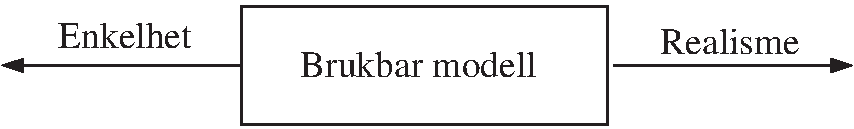
\includegraphics[scale=0.7]{figurer/fig1_1.pdf} 
 \caption{Status av en modell}
	\label{fig:status_modell}
\end{figure}
\noindent
Vi vil derfor aldri si at en modell er den riktige modell.
Vi begrenser oss til å si at en modell ser ut til å være mer
velegnet enn andre modeller.  Praktisk erfaring er det eneste som kan gi en
pekepinn om dette. 

Modeller blir brukt i alt fra vitenskap til spekulativ virksomhet.
Dersom en i vitenskapen hevder at visse observerte
fenomener kan tilfredsstillende forklares ved hjelp av en bestemt modell, 
så kan andre interesserte studere fenomenet for å etterprøve dette.
Har en modell overlevet mange etterprøvinger, tas dette til inntekt for at
modellen er brukbar og har gitt oss felles innsikt.
I økonomisk virksomhet kan gode modeller gi bedre beslutninger, og 
målbare gevinster.

Det er vanlig å skille mellom to hovedtyper av modeller,
{\em deterministiske modeller} og {\em stokastiske modeller}. En
deterministisk modell betrakter en iakttakelse eller et utfall
som entydig bestemt ut fra gitte eksperimentbetingelser. Dersom modellen er
realistisk vil vi, såframt vi har godt kjenn\-skap til disse, kunne bruke
modellen til å forutsi utfallet med stor grad av sikkerhet. 
Mange iakttakelser er av en slik natur at det ikke lar seg gjøre å
finne en brukbar deterministisk modell.  La oss illustrere dette med et
eksempel :

Anta at vi skyter en terning ut av en kanon utover en horisontal flate. 
Dersom vi bare er interessert i å iaktta posisjonen hvor terningen treffer
bakken, så er det lett å lage en brukbar deterministisk modell
basert på Newtons andre lov, dvs. kraft er lik masse ganger
akselerasjon K=m$\cdot$a.  Dersom vi bare er interessert i hvilken side
av terningen som vender opp når den har falt til ro, vil det være
verdiløst å prøve å lage en deterministisk modell (selv om en
slik eksisterte) basert på Newtons bevegelseslover.  Like\-vel vil
det være ønskelig å lage en slags modell for eksperimentet, helst
en modell som tar hensyn til forestillingen om at alle 6 sider på
terningen har samme sjanse for å vende opp.  Modeller som er
ikke-deterministiske og inne\-holder forestillinger om usikkerhet
og variasjon, kaller vi {\em stokastiske modeller}. 
Ordet stokastisk er avledet av det greske ord for tilfeldighet. 

Typisk for mange fenomener i praksis er usikkerhet og variasjon, enten ved at
vi har begrenset informasjon, eller ved at det fenomen vi studerer selv
varierer. I denne sammenheng skal modeller blant annet hjelpe oss til å
\begin{itemize}
\item    finne sammenhenger som vi ikke så tidligere,
\item    relatere virkninger og mulige årsaker,
\item    forstå variasjon,
\item    gjøre usikkerhetsvurderinger.
\end{itemize}                             

Mange praktiske og teoretiske problemer
innenfor en rekke fagområder lar seg best analysere ved
hjelp av stokastiske modeller.  Dette betyr ikke at vi aksepterer at
naturen spiller hasard, men at en stokastisk modell kanskje er det eneste
av praktisk nytte.  Stokastiske modeller er i dag et viktig
verktøy i mange vitenskaper såvel som i teknologi og økonomisk
virksomhet. Heldigvis er en stor del av den grunnleggende teori for slike modeller
felles for anvendelser innen de fleste fag- og anvendelsesområder, og 
denne boka gir innblikk i sentrale elementer i slik teori.


\section{Sannsynlighet}

Sannsynlighetsregning er en gammel disiplin, den første tid 
motivert ut fra ønsket om å analysere veddemål knyttet til
myntkast, terningsspill, kortspill etc.  Det er kjent at
Fermat, Pascal og Huygens syslet med sannsynlighetsbegrepet på midten av
1600-tallet, Cardano allerede hundre år før.  To milepeler i 
klargjøring av sannsynlighetsbergrepet var
utgivelsen av Jacob Bernoullis arbeid ``Ars conjectandi'' (Kunsten
å gjette) i 1713 og  deMoivres ``Doctrine of chances'' i 1718.
I  1763 lanserte Thomas Bayes et subjektivistisk sannsynlighetsbegrep 
i sitt ``Essay towards solving a problem in doctrine of chance''. 

Etterhvert dukket behovet for å snakke om og regne med
sannsynligheter opp på stadig flere områder. Dette krevde et
bedre teoretisk fundament. Russeren Kolmogorovs aksiomatiserte 
sannsynlighetsbegrepet i et arbeid fra 1933, og dette
ga støtet til intens utvikling av sannsynlighetsteori på resten av 
1900-tallet. Parallelt med dette fikk subjektivistiske id\'{e}er 
sin renessanse anført av Ramsey, De Finetti og Savage med flere.

La oss ved hjelp av noen enkle eksempler prøve å nærme oss
sannsynlighetsbegrepet på rent intuitivt grunnlag.\\

\begin{eksempel}{Myntkast}
Vi kaster et kronestykke og observerer enten kron eller mynt. 
Spørsmål:  Hva er sjansen for henholdsvis kron og mynt?  De aller
fleste vil vel svare at sjansen for hvert av utfallene er 1/2. 
Noen vil kanskje uttrykke seg annerledes og si at sjansen er
``fifty-fifty'' eller oddsene er 1 : 1, men dette er i realiteten
det samme.  La oss avkreve begrunnelser:  Person $A$ begrunner sitt
utsagt med å si at hvert av de 2 mulige utfall må ha samme sjanse
for å inntreffe, og sjansen for kron må derfor være lik 1/2. 
Person $B$ begrunner sitt utsagn med å si at dersom en knipser
mynten et stort antall ganger, vil kron opptre i omtrent halvparten 
av forsøkene.  $A$ sier at han har benyttet sin teoretiske
abstraksjonsevne vedrørende konstruksjonen av et kronestykke,
mens $B$ sier at hun har brukt sin praktiske erfaring i myntkast. 
De to begrunnelsene er derfor fundamentalt forskjellige, men
begge kan aksepteres.  De fleste vil vel si at det skulle være
unødvendig å gjøre noen praktiske eksperimenter i det hele tatt
for å kunne konkludere at sjansene er ``fifty-fifty''.
\end{eksempel}
                          
De første famlende forsøk på å definere et sannsynlighetsbegrep
tok derfor utgangspunkt i id\'{e}en om like mulige utfall ($A$'s
argument).  Dette var tilfredsstillende så lenge en bare var
interessert i å anvende det på spill, men allerede neste eksempel
viser at et slikt sannsynlighetsbegrep er for snevert.\\

\begin{eksempel}{Kast med tegnestift}
Ta en tegnestift og kast den ut på bordet.  Spørsmål:  Hva er
sjansen $p$ for at den faller til ro med spissen opp?  Vi ser at
det også er to mulige utfall av dette eksperimentet.  Argumentet
$A$ benyttet i Eksempel 1 lyder nå:  De to utfallene er like
sannsynlige, ergo er sjansen 1/2 for at spissen peker opp.  Dette
argumentet har vel liten appell her, de fleste vil nok avvise
det.  Det er ikke lett å se hvordan vi ved å granske tegnestiftens
 konstruksjon, skal kunne si noe om sjansene for de to
utfallene.  For å skaffe seg litt innsikt i tegnestiftens
egenskaper, tenker vi oss at $A$ og $B$ hver for seg har kastet
tegnestiften $n$=100 ganger.  La oss betegne resultatet at stiften
faller til ro med spissen opp med $r_{1}$ og resultatet at den faller
til ro med spissen ned med $r_{2}$.  $A$ har observert $n(r_{1})=47$,
$n(r_{2})=53$, mens $B$ har observert $n(r_{1})=42$, $n(r_{2})=58$ ($n(\cdot )$
 betyr ``antall ganger'').  Den relative hyppighet av hvert av resultatene ble \\

For $A$:
\[h(r_{1}) = \frac{n(r_{1})}{n} = \frac{47}{100} = 0.47  \ , \
 h(r_{2}) = \frac{n(r_{2})}{n} = \frac{53}{100} = 0.53 \] 

For $B$:                        
\[h(r_{1}) = \frac{n(r_{1})}{n} = \frac{42}{100} = 0.42 \ , \
 h(r_{2}) = \frac{n(r_{2})}{n} = \frac{58}{100} = 0.58 \] 

\noindent
Dersom andre kaster den samme tegnestiften et stort antall ganger
(f.eks. 100), ville hver trolig observere relative hyppigheter nær
opp til disse.  Hvilken erfaring kan en så i fall trekke av våre
eksperimenter? :
\begin{itemize}
 \item
  Dersom vi utfører en rekke forsøksserier med mange forsøk i
     hver serie, så vil den relative hyppighet av hvert
     forsøksresultat være omtrent den samme i hver av
   forsøksseriene såframt forsøksbetingelsene ellers er de samme.
\end{itemize}

\noindent På bakgrunn av sine erfaringer uttalte $A$ at sjansen for at
tegnestiften faller til ro med spissen opp er $p=0.47$, mens $B$
påsto at sjansen var mindre, nemlig $p=0.42$.  For ikke å bli
uvenner på grunn av en tegnestift, ble $A$ og $B$ enige om å kaste
stiften 300 ganger til i fellesskap.  Det viste seg at spissen
pekte opp i 225 av de i alt $n=500$ kastene, de fikk altså

\[h(r_{1}) = \frac{n(r_{1})}{n} = \frac{225}{500} = 0.450 \ , \ 
 h(r_{2}) = \frac{n(r_{2})}{n} = \frac{275}{500} = 0.550 \] 
På bakgrunn av sine samlede erfaringer anslår $A$ og $B$ at sjansen
for at spissen peker opp er $p=0.45$.  Dersom de fortsatte å kaste
tegnestiften, er det lite trolig at det noen gang blir nødvendig å
endre dette anslaget i særlig grad.  Denne $p$ oppfatter en
derfor som en egenskap ved tegnestiften.  Selv om den valgte verdi av $p$ er
funnet som en relativ hyppighet for et stort antall gjentakelser av
eksperimentet, tyder all erfaring på at denne verdien også har
relevans for et rasjonelt menneskes holdning til et lite antall kast,
sogar et enkelt kast.  Den ``sanne verdi av $p$'' vil aldri kunne bli eksakt
kjent.  Likevel viser det seg fruktbart å bygge modeller basert
på forestillingen om en slik verdi.  En nærmere analyse som vi
vil bli i stand til å utføre senere vil vise at vi, selv med
$n=500$, ikke kan være trygg for at siste sifferet i $p=0.45$ vil
være ``korrekt'', $n$ er faktisk ikke stor nok til det.
\end{eksempel}                                                             

Enkelte forsøker å definere sannsynligheten $p$ for
et bestemt utfall av et eksperiment som grenseverdien for den
relative hyppighet av utfallet i en serie av $n$ uavhengige
gjentakelser av eksperimentet, under de samme betingelser,
når $n$ går mot uendelig.  Neste eksempel viser at dette
er for snevert.\\
                            
\begin{eksempel}{Fødsel og død}
Eva skal føde for første gang, og spør seg selv om sjansene for
henholdsvis gutt eller pike.  Hun har hittil forestilt seg at
sjansene er ``fifty-fifty'', men leser en dag i avisen av
hyppigheten av guttefødsel og pikefødsel i Norge for tiden er  
henholdsvis 0.514 og 0.486.  Disse hyppighetene kan ikke uten
videre betraktes som en egenskap ved Eva, hun utfører jo sitt
``eksperiment'' for første gang (sml. tegnestifteksperimentet). 
Likevel mener Eva at tallene også er relevant for henne, og andre i samme
situasjon. Med litt velvillighet vil en kanskje si at tallene ovenfor kan
tolkes som relative hyppigheter i et stort antall gjentakelser av samme
eksperiment, og at de uttrykker en egenskap ved den kjønnsbestemmende
mekanisme hos mennesker.  Som i forrige eksempel kan det
være naturlig å definere sannsynligheter som idealiserte
relative hyppigheter.  Imidlertid ser vi at en slik definisjon
innebærer visse vansker.  For det første er det
umulig å gjenta dette eksperimentet et ubegrenset antall ganger. 
Vi får også problemer med hvor langt vi kan tøye begrepet samme
eksperiment.  Tenk bare igjennom følgende: 
Hva er sjansen $p$ for at den nyfødte overlever sin 70-årsdag?  En
rekke faktorer som helsetjeneste, kosthold og livsstil varierer, og dette
gjør definisjonen vanskelig. 
Likevel er det uhyre fruktbart å tenke seg modeller
med forestillinger om en ``sann'' $p$, og det finnes statistiske 
metoder som kan gi brukbare anslag for denne $p$, som kan gi grunnlag for
fornuftige beslutninger.
\end{eksempel}

\begin{eksempel}{Snø og ski}
Ski er en kjær julegave for småbarn, også i Bergen.  Bergenske
sports\-handlere har erfart følgende problem :  Dersom det faller
snø før jul, resulterer dette i voldsom etterspørsel etter
barneski i ukene før jul.  Dersom julesnøen uteblir, er
etterspørselen minimal, og heller ikke når snøen kommer vil salget
nå de store høyder.  Anta at bestillinger til fabrikkene må
være inne før 1. august.  Problemet for vår sportshandler vil
være hvor mange skipar han bør bestille.  Et naturlig spørsmål
å stille seg da er:  Hva er sjansen for julesnø i år?  For å
svare på dette spørsmålet kan sportshandleren selvsagt ty til
nedtegnede data over nedbørforholdene i Bergen før jul tidligere år. 
Det kan også være aktuelt å gjøre bruk av andre opplysninger,
for eksempel langtidsvarsler fra Meteorologisk institutt.
\end{eksempel}


\begin{eksempel}{Bookmaking}
En bookmaker tilbyr veddemål omkring utfallet av cupfinalen i
fotball mellom Lyn og Brann.  Anta at han er kommet fram til at
odds er 3 til 1 i favør av Brann.  Dette betyr at han tror at
sjansen for at Brann vinner er 3/4, mens sjansen for at Lyn
vinner er 1/4.  For å komme fram til dette resultat har han
vurdert lagenes prestasjoner i de siste kampene de har spilt, de
siste innbyrdes oppgjør.  Videre har han tatt i betraktning
lagenes formkurve, antall menn på sykelisten, lagenes lagmoral
for øyeblikket.  Det er ikke grenser for momenter som kan trekkes
inn, og en bookmakers vurdering av odds vil derfor være svært
subjektiv.
\end{eksempel}

I alle disse 5 eksemplene har det vært naturlig å snakke om
sjanser eller sannsynligheter.  Men vi har ikke kommet til
klarhet i hvordan et fruktbart sannsynlighetsbegrep bør defineres,
spesielt ikke dersom vi ønsker at slike problemer som er
nevnt i Eksempel 4 og 5 skal falle innenfor rammen av begrepet. 
Det har ofte stått strid om hvor langt en kan tøye 
sannsynlighetsbegrepet.  Noen forfekter et subjektivt eller
personlig sannsynlighetsbegrep, dette i motsetning til forestillingen
om at en sannsynlighet bør være noe objektivt ved det
fenomen som studeres, uavhengig av personen som beregner denne
sannsynligheten.  Begge syn har sine fordeler og ulemper, men vi
skal ikke ta stilling her.  Vi skal innføre
sannsynlighetsbegrepet aksiomatisk, dvs. vi stiller opp de minstekrav
som må være oppfylt for at den struktur vi arbeider med skal kunne
kalles en sannsynlighetsmodell. Dette teorigrunnlaget legges
Kapittel 2, og utvikles videre i etterfølgende kapitler.
           

\section{Statistikk}

Dersom man ber en statistiker av i dag om å gi en kort definisjon
av sitt fag, er det mulig at svare er:

\begin{quote}
Statistikk $=$ Id\'{e}er og metoder for å forstå variasjon
\end{quote}

\noindent I en norsk fremmedordbok leser vi imidlertid at
statistikk er:

\begin{enumerate}
\item Systematisk innsamling og tabellering av tallmessige forhold.
\item Vitenskap om belysningen av visse masseforeteelser i
     samfunnet bygd på tallmessige oppgaver (f.eks. fødsler,
     dødsfall, forbrytelser osv.).
\end{enumerate}

\noindent Dette samsvarer kanskje med hva folk legger i ordet
statistikk, men la oss se hvordan ordet etter hvert har fått en
 videre betydning.
                                 
Går vi tilbake i historien for å finne opprinnelsen til fagfeltet
statistikk, nevnes ofte et arbeid av engelskmannen John Graunt
som ble publisert i 1662 med tittelen ``Natural and political
observations ... made upon the bills of mortality''.  På 1700 og
1800 tallet ble det i flere land vakt en interesse for å foreta
systematisk innsamling og bearbeiding av data om befolkning,
handel, jordbruk osv., eller kort og godt om rikets tilstand. 
Ordet statistikk er da også avledet av det latinske ord for
tilstand (sml. det engelske ``state'').  Også i dag er dette en
viktig del av det statistiske arbeids\-feltet, og fagfolk kaller
dette for {\em deskriptiv} (eller {\em beskrivende}) {\em statistik}k.

Det har imidlertid ingen hensikt å samle inn data med mindre de
brukes til noe.  Etter hvert ble statistikerne interessert i
generelle prinsipper for tolkning av statistiske data, om hvordan
slike data kan benyttes til å slutte noe ut over dataene selv, 
ofte kalt {\em statistisk inferens}. 
Statistikk utviklet seg som eget fag {\em teoretisk statistikk}. 
De første forløpere til
moderne statistisk teori finner vi hos matematikerne Gauss og
Laplace på begynnelsen av 1800-tallet.  Disse laget en teori for
analyse av målefeil ved fysiske observasjoner.  Det neste
avgjørende puff kom i de første tiår etter 1900. Sentrale personer i
pion\'{e}rtiden  da statistikk utviklet seg som eget fag var Karl Pearson,
Ronald A. Fisher og Jerzy Neyman.  Utviklingen
skjøt raskt fart, og den skjedde i kontakt med såvel matematikken,
som naturvitenskapene og samfunnsvitenskapene.  Fra 1950-årene 
begynte mange statistikere å oppfatte fornålet med sitt fag som det 
å etablere prinsipper for beslutning under usikkerhet. I dag er få
så ambisiøse, men ønsker en å fremheve dette aspektet brukes gjerne 
betegnelsen {\em statistisk beslutningsteori}.

Statistikkfaget har vært i kontinuerlig utvikling gjennom hele 1900-tallet,
med tilfang av stadig nye metoder. 
Praktiske problemer fra jordbruk, industri og økonomi ledet ofte til ny
teori som alle kunne dra nytte av, og som derfor har blitt felleseie for mange ulike 
fagområder og anvendelser. Statistikk som fag er blitt kalt 
``The servant of all sciences'' og ``The accounting discipline for scientific credibility``.

Moderne statistisk teori er i hovedsak basert
på stokastiske modeller og sannsynlighetsregning. Mange aktuelle analysemetoder 
er uten slik teoretiske forankring. Det gjelder spesielt 
metoder for såkalt {\em eksplorativ dataanalyse}, ved slutten av 1990-tallet
markedsført under merkelappen ``data mining''. Dette felt er ikke dekket i denne boken.

De følgende eksempler tar sikte på å gi leseren et innblikk i
noen sentrale statistiske problemstillinger.  Vi håper at disse
kan gi leseren en viss motivasjon for å gi seg i kast med
statistisk teori, samt forstå nødvendigheten av basiskunnskaper i
sannsynlighetsregning.  Lesere som primært er interessert i
sannsynlighetsregning kan gå direkte løs på Kapittel 2, og
eventuelt heller lese dette stoffet som en opptakt til Kapittel 7
og 8.\\

\begin{eksempel}{Måleproblemer - tilfeldig variasjon}
En bedrift er interessert i kvaliteten av artikler produsert
etter en nyutviklet metode, og som et eksperiment prøveproduseres
i alt n=50 artikler, hvoretter kvaliteten måles.  Kvalitet kan
f.eks. være den belastning i kilo som artiklen tåler inntil den
går i stykker.  Resultatet ble (med en desimal)

 \begin{center} 
 \begin{tabular}{cccccccccc}
  2.9 & 2.7 & 3.1 & 2.8 & 2.8 & 2.7 & 2.9 & 3.0 & 2.6 & 3.1  \\
  3.1 & 3.0 & 2.8 & 2.9 & 2.7 & 2.9 & 3.0 & 2.6 & 3.2 & 2.9  \\
  2.7 & 2.8 & 3.1 & 3.1 & 2.9 & 2.9 & 2.8 & 3.4 & 3.0 & 2.8  \\
  3.0 & 2.9 & 2.7 & 3.2 & 2.8 & 3.1 & 2.4 & 2.9 & 3.2 & 2.9  \\
  3.1 & 3.3 & 2.9 & 2.9 & 2.8 & 2.7 & 2.8 & 2.8 & 3.1 & 3.0  \\
 \end{tabular}
\end{center}

\noindent For å skaffe oversikt over dette tallmaterialet lages en
{\em hyppighetstabell}

\begin{center}  \small \addtolength{\tabcolsep}{-0.4\tabcolsep}
 \begin{tabular}{l|ccccccccccc}
Verdi     & 2.4&2.5&2.6&2.7&2.8&2.9&3.0&3.1&3.2&3.3&3.4 \\ \hline
Hyppighet & 1 & 0 & 2 & 6 & 10 & 12 & 6 & 8& 3& 1 & 1 \\
Relativ hyp.&0.02&0.00&0.04&0.12&0.20&0.24&0.12&0.16&0.06&0.02&0.02 \\ \hline
 \end{tabular}
\end{center}
           
Tabellen gir utrykk for en kvalitetsfordeling:  kvaliteten kan
variere, men noen verdier er mer typiske enn andre.
Mer instruktivt er å lage et {\em histogram}, se Figur~\ref{fig:histogram}. Her er
tegnet søyler svarende til hver av kategoriene i
hyppighetstabellen, med areal proporsjonalt med de respektive hyppigheter,
se Figur~\ref{fig:histogram}.
\begin{figure}[ht]
\centering \centering
\includegraphics[scale=0.8]{figurer/fig1_2.pdf}
 \caption{Histogram}  
	\label{fig:histogram}
\end{figure}                           

En størrelse av betydelig interesse vil være den gjennomsnittlige
kvalitet, som i dette tilfellet er 2.914.  I tillegg til
gjennomsnittet ønskes ofte et mål for variasjonen i kvalitet.  Et
slikt mål er variasjonsbredden, som her er 1.0.  Et alternativt
mål er standardavviket (defineres nedenfor), som her beregnes til
0.191.  Dette gir i større grad enn variasjonsbredden uttrykk for
et ``typisk'' avvik fra gjennomsnittet.
\end{eksempel}

La oss generelt tenke oss et observasjonsmateriale bestående av $n$
observasjoner

                  \[X_{1}, X_{2}, X_{3}, \ldots ,X_{n}\]
                 
\noindent {\em Gjennomsnittet} (middeltallet) av observasjonene er da gitt ved
                                     
  \[\bar{X} = \frac{1}{n}(X_{1}+X_{2}+X_{3}+ \cdots +X_{n}) =
\frac{1}{n} \sum_{i=1}^{n}X_{i}\]

\noindent mens {\em standardavviket} til observasjonene er gitt ved

\[S_{X} = \sqrt{ \frac{1}{n}\sum_{i=1}^{n}(X_{i}-\bar{X})^{2}}\]


\noindent $S_{X}^{2}$ kalles ofte for {\em variansen} til observasjonene.
Presentasjon av
hyppighets\-tabeller, histogrammer, gjennomsnitt og standardavvik
osv. tar sikte på å få fram typiske trekk ved et tallmateriale.
Disse og andre grafiske og numeriske presentasjonsformer
faller under betegnelsen beskrivende statistikk.

I mange situasjoner er vi interessert i å gjøre noe mer enn bare
å beskrive tallmaterialet, vi ønsker kanskje å bruke resultatene
i planlegging, som grunn\-lag for prognoser eller beslutninger.  Da
melder det seg en rekke spørsmål, og la oss diskutere noen av
disse med utgangspunkt i eksemplet ovenfor:

Vi ønsker typisk å uttale oss om kvaliteten av artikler dersom vi
fortsetter å produsere etter samme metode.  I denne forbindelse
er det naturlig å tenke seg at metoden generelt kan tillegges en
``sann'' kvalitetsfordeling, dvs. at ``i det lange løp'' er andelen
av de ulike kvaliteter bestemt av metoden selv.  Det viser seg
fruktbart å tenke på disse andelene som sannsynligheter, og
kvalitetsfordelingen som en såkalt {\em sannsynlighetsfordeling}. 
Slike sannsynligheter kan danne utgangspunkt for ulike beregninger,
og for dette formål kan vi ha nytte av å teori
for sannsynlighetsregning.  Sannsynligheter kan blant annet
brukes til å si noe om kvaliteten ved produksjon av et gitt
antall artikler, f.eks. sjansen for at et parti på 10 artikler
ikke inneholder artikler under en viss kvalitet.  Slik
sannsynlighets\-regning forutsetter at de ``sanne'' sannsynlighetene er
kjente.  I praksis er dette sjelden tilfelle, og spørsmålet er da
hvordan vi kan bruke informasjonen fra prøveproduksjonen
til å trekke konklusjoner om de teoretiske sannsynlighetene.

En problemstilling som har spesiell interesse er følgende:  Vi
tenker oss at produksjonsmetoden kan karakteriseres ved et
kvalitetsnivå $\mu$ som gir uttrykk for gjennomsnittlig kvalitet
``i det lange løp``.  Hver observasjon i prøveproduksjonen oppfattes
som en observasjon av dette nivå, men som pga. tilfeldigheter kan
avvike noe fra dette, såkalt {\em tilfeldig variasjon}. 
Sannsynlighetsfordelingen kan brukes som et uttrykk for sjansene for at
en enkelt observasjon faller i de ulike kvalitetskategorier, og     
kvalitetsnivået $\mu$ oppfattes som {\em forventet} kvalitetsnivå.  I
praksis vil forventningen $\mu$ ofte være ukjent, og formålet med å
foreta observasjoner, er bl.a. å skaffe informasjon om denne. Svært
ofte blir middeltallet $\bar{X}$ brukt som anslag på forventningen $\mu$.
       
Av spørsmål som en kunne ønske å få besvart nevner vi: 
Hvilke feil\-mar\-giner  må man regne med dersom vi anslår forventningen
på denne måten?  Her hadde vi femti observasjoner, men hva dersom vi
hadde bare fem?  Hvor mange observasjoner må vi innhente dersom
vi ønsker en viss feilmargin?  Gir observasjonene grunnlag for å
påstå at forventningen er mindre enn (større enn) 3.0?  Hva er
sjansen for feilaktig å påstå noe slikt osv.  For å besvare
spørsmålene trengs statistisk teori.  Vi formulerer da de
antakelser vi er villig til å gjøre om observasjonene i en
statistisk mo\-dell, og utleder våre konklusjoner ut fra denne.  En
aktuell modell i denne forbindelse er den såkalte {\em målemodellen}
som blir diskutert i Kapittel 8.  En del grunnleggende begreper
som trengs blir utviklet i Kapitlene 3-6.\\
                                     
\begin{eksempel}{Stikkprøver - pålitelighet}
Vi ønsker å finne ut noe om tilbøyeligheten til å bære på
kontanter for en gruppe studenter.  Det er tungvint
å innhente opplysninger fra alle studentene (populasjonen).  I     
steden trekkes en stikkprøve (et utvalg) på et mindre antall
studenter, og vi ønsker å trekke konklusjoner om tilbøyeligheten
blant alle studentene på grunnlag av opplysninger fra utvalget. 
Hvilken pålitelighet kan vi tillegge generelle konklusjoner
basert på slike stikkprøver?

La oss se på en tenkt situasjon der populasjonen består av et
kull på $N$=216 studenter.  Anta at kronebeløpene til disse
studentene er (rekkefølgen er likegyldig) :


\begin{center}                                                              
\begin{tabular}{|rrrrrr|rrrrrr|}   \hline
 80& 93& 65&328& 10& 28&113&476& 57& 54& 13& 21 \\
232& 56& 49& 35&  5& \underline{0}&280& 37&376& 24& 36& 51 \\
 26&155& 62&237&532& 19& 56&112& 40&136& 53&263 \\        
 97&206&  4&286&134&  8&\underline{145}&500&164& 41&178&\underline{285} \\
 91&113&262& 47&  6&188& 48& 26& 29& 45& 94&100 \\
620& 79&306& 59& 55&136& 29&175&113& 35& 40&383 \\ \hline                   
 17&452&110&  8&109&\underline{273}&114& 46&170&481& 38&719 \\
 25&  0&381&139&153& 36&242& 59& 78& 72&380& 87 \\
192& 57&123& 81& 13& 30&  \underline{0}& 51&184& 98&  0&\underline{312} \\
771& 27& 40& 99& 90&206&214& 12&317&119&152& 11 \\
  0& 19&113& 59& 31& 37& 22& 14& 73&310& 81&341 \\
 17& 86& 63&  7&212& 45&110& 72&637& 46&118& 26 \\ \hline
\underline{51}&312& 59& 86&110&145& 74&\underline{  8}&\underline{411}& 71&450& 23 \\
176&253& 21& 98& 43& 36&145& 60&427& 78& 83& 85 \\
119&  9&276& 34& 12&180&277&185& 27& 13&412& 64 \\
 53& 53& 78&291& 85&578&370&479& 85&  0&110&174 \\
\underline{ 7}&176&130&109& 49&345& 49&156&111& 78& 91&373 \\
 55&222& 91&846& 19& 64& 62&274&318&185&200&502 \\ \hline
 \end{tabular}
\end{center}
                                             
                                       
\noindent Disse tallene er i utgangspunktet ukjente for oss, men la oss likevel
se litt nærmere på dem, for å forstå hva som kan
hende ved analyse av stikkprøver.

La oss først se på hyppighetsfordelingen av pengebeløpene. 
Siden antall ulike beløp som forekommer er svært stort, 
får vi bedre oversikt dersom vi grupperer beløpene , f.eks. slik

\begin{center} 
 \begin{tabular}{l|cccccc}
Beløp  & 0-99 & 100-199 & 200-299 & 300-399 & 400-499 & 500-  \\ \hline
Hyppighet & 121&   43    &   19    &   16    &    8    &   9    \\
Relativ hyp.& 0.56  & 0.20 &  0.09 &  0.07  &  0.04  & 0.04  \\ \hline
 \end{tabular}
\end{center}

\noindent Vi kunne alternativt bruke en finere gruppering, men den vi har
valgt fanger likevel opp de karakteristiske trekk ved materialet. 
Et histogram vil i denne situasjonen se ut som i Figur~\ref{fig:hist_grupperte}.                   
            
\begin{figure}[ht]
\centering\centering 
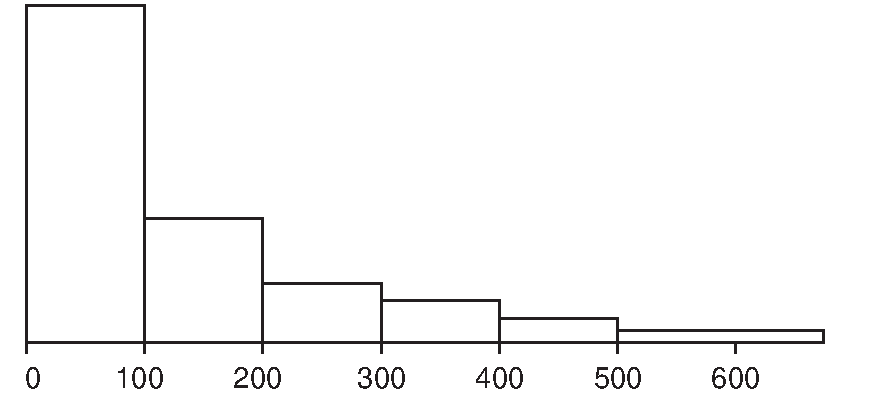
\includegraphics[scale=0.7]{figurer/fig1_3.pdf}
 \caption{Histogram grupperte data}
	\label{fig:hist_grupperte}
\end{figure}

Vi ser at denne fordelingen er nokså ulik den i foregående
avsnitt, den er skjev med hovedmassen av kronebeløpene mellom 0
og 100.  Gjennomsnitt\-lig kronebeløp beregnes her til 144.20, mens
standardavviket er beregnet til 155.20.  Det gjennomsnittlige
beløp er altså langt over det beløp som majoriteten har på seg,
som skyldes at enkelte studenter bærer på relativt store
beløp.  Vi ser at betydelig variasjon mellom studentene
innbyrdes kommer til uttrykk ved et relativt høyt standardavvik. 
I en slik situasjon vil alternative beskrivende mål ha interesse.
Et slikt er {\em medianen}, som er det kronebeløp som er slik at like
mange studenter har mer og mindre enn dette beløp.  I tallmaterialet
ovenfor er kr. 85.50 en median.                   

La oss nå tenke oss at situasjonen er slik at tallene ovenfor
alle er ukjente for oss, og at vi ønsker å finne ut noe om
tilbøyeligheten til å bære med seg penger ut fra en stikkprøve
på, la oss si $n$=10 tilfeldig utvalgte studenter.  Anta at
studentene er nummerert fra 1 til 216 (rekkefølgen er likegyldig),
og at vi ved hjelp av en upartisk mekanisme trekker ut ti studenter
(vi kan f.eks. gjøre bruk av en terning).  Resultatet ble de studenter
som er understreket i tabellen, og deres kronebeløp er:

\begin{center} 
 \begin{tabular}{lcccccccccc}                                         
 Beløp :&  0 &  145 &  285 &  273 &  0 & 312 &  51 &  8 & 411 & 7
 \end{tabular}
\end{center}


\noindent Anta at vi primært er interessert i gjennomsnittlig pengebeløp
blant alle studentene.  Det synes rimelig å bruke gjennomsnittet
i utvalget som anslag på gjennomsnittet i hele populasjonen.  Med
vårt utvalg beregner vi gjennomsnittet til 149.2, og spørsmålet
er i hvilken grad dette gir pålitelig informasjon om det
virkelige gjennomsnittet.

At usikkerheten ved en stikkprøve av den gitte størrelsesorden
kan være betydelig, kan bekreftes ved å ta en ny stikkprøve på 10
studenter.  Denne gangen fikk vi et gjennomsnitt i utvalget på
107.5.  Det faktum at vårt opp\-rinne\-lige anslag 149.2 er nær
gjennomsnittet i populasjonen 144.2 beror derfor på flaks, det er
betydelig risiko for at stikkprøven gir et anslag som er mye mer
avvikende.
           
I praksis vet vi jo ikke hva gjennomsnittet eller medianen i
populasjonen er, og vi kan da stille spørsmål av typen:  Hva er
sjansen for at et anslag basert på en stikkprøve er høyst 50
kroner feil?  etc.  Det viser seg at svaret på slike spørsmål vil
avhenge av stikkprøvens størrelse, populasjonens størrelse og
struktur, spesielt har variabiliteten av verdiene i populasjonen
betydning.  For å vurdere hvordan alt dette påvirker
påliteligheten av stikkprøver, trenger vi teoretiske
kunnskaper.  En teoretisk modell i denne forbindelse er den
såkalte {\em lotterimodellen} som beskrives i Kapittel 8.  Den
forutsetter at stikkprøven er et såkalt {\em tilfeldig utvalg}, et
begrep som tas opp i Kapittel 3. Mer omfattende teorier for
utvalgsundersøkelser tas opp i Kapittel 14 og 15.
\end{eksempel}

\begin{eksempel} {Samvariasjon - korrelasjon}
I mange statistiske undersøkelser foreligger sammenhørende
observasjoner av to eller flere variable, og formålet er å
klargjøre en eventuell sammenheng mellom disse.  Vi vil her ta
utgangspunkt i et eksempel med to variable:
             
Ved avsluttende siviløkonomeksamen ved NHH våren 1967 var det 91
studenter oppe til eksamen i samfunnsøkonomi (S) og
bedriftsøkonomi (B).  Karakterene var (karaktersystem: 0 til 9,
med 9 som beste karakter):
\begin{center}   
 \begin{tabular}{|cc|cc|cc|cc|cc|cc|cc|} \hline
S & B & S & B & S & B & S & B & S & B & S & B & S & B \\ \hline
8 & 6 & 5 & 5 & 5 & 4 & 6 & 5 & 5 & 8 & 7 & 7 & 6 & 6 \\
3 & 5 & 5 & 6 & 5 & 6 & 3 & 6 & 3 & 6 & 7 & 5 & 7 & 5 \\
7 & 6 & 6 & 4 & 4 & 4 & 5 & 4 & 3 & 6 & 4 & 5 & 6 & 6 \\
4 & 4 & 3 & 4 & 6 & 6 & 8 & 6 & 6 & 5 & 6 & 5 & 7 & 6 \\      
5 & 4 & 3 & 4 & 7 & 6 & 5 & 5 & 4 & 5 & 4 & 4 & 6 & 6 \\
4 & 6 & 8 & 6 & 5 & 5 & 7 & 5 & 4 & 4 & 4 & 4 & 5 & 6 \\
5 & 5 & 5 & 7 & 3 & 6 & 7 & 5 & 5 & 6 & 5 & 6 & 4 & 3 \\
6 & 3 & 8 & 7 & 6 & 5 & 6 & 7 & 8 & 8 & 6 & 6 & 7 & 5 \\
3 & 3 & 6 & 5 & 3 & 6 & 7 & 3 & 9 & 5 & 5 & 4 & 4 & 5 \\
7 & 5 & 6 & 5 & 3 & 6 & 3 & 5 & 4 & 5 & 4 & 6 & 4 & 4 \\
3 & 5 & 5 & 5 & 4 & 4 & 7 & 8 & 5 & 6 & 8 & 5 & 4 & 6 \\
3 & 4 & 4 & 6 & 7 & 3 & 7 & 8 & 4 & 4 & 5 & 5 & 5 & 5 \\
4 & 3 & 7 & 5 & 7 & 5 & 5 & 6 & 4 & 2 & 3 & 6 & 1 & 4 \\ \hline
 \end{tabular}
\end{center}
                            
\noindent
En bedre oversikt over materialet får vi dersom vi lager en
todimensjonal hyppighetstabell. Denne uttrykker den 
{\em simultane hyppighetsfordeling} av
samfunns\-øko\-nomi og bedriftsøkonomikarakter for denne gruppen studenter. 
Summeres linjevis og kolonnevis får vi de {\em marginale hyppighetsfordelinger}
for henholdsvis samfunns- og bedriftsøkonomi.

            
\begin{center}                 
 \begin{tabular}{|c|cccccccccc|c|} \hline
Samf.-    &  \multicolumn{10}{c|}{Bedriftsøkonomi}&   \\ \cline{2-11}
øk.    & 0 & 1 & 2 & 3 & 4 & 5 & 6 & 7 & 8 & 9 & Sum \\ \hline
  0       &   &   &   &   &   &   &   &   &   &   &  0   \\
  1       &   &   &   &   & 1 &   &   &   &   &   &  1   \\
  2       &   &   &   &   &   &   &   &   &   &   &  0   \\
  3       &   &   &   & 1 & 3 & 3 & 7 &   &   &   & 14   \\
  4       &   &   & 1 & 2 & 8 & 4 & 4 &   &   &   & 19   \\
  5       &   &   &   &   & 4 & 7 & 7 & 1 & 1 &   & 20   \\
  6       &   &   &   & 1 & 1 & 6 & 5 & 1 &   &   & 14   \\
  7       &   &   &   & 2 &   & 8 & 3 & 1 & 2 &   & 16   \\
  8       &   &   &   &   &   & 1 & 3 & 1 & 1 &   &  6   \\
  9       &   &   &   &   &   & 1 &   &   &   &   &  1   \\ \hline
Sum       & 0 & 0 & 1 & 6 &17 &30 &29 & 4 & 4 & 0 & 91   \\ \hline
  \end{tabular}                
\end{center}  
                                                                    
\noindent                          
Hyppighetstabellen gir et visst inntrykk av (positiv) samvariasjon mellom
de to karakterene, studenter med god karakter i
samfunn har også gjennomgående bra karakter i bedrift og omvendt. 
På den annen side finnes også enkelte ``spesialister''.  Vi kunne
ønske oss et numerisk mål for graden av samvariasjon mellom de to
karakterene i tallmaterialet.
\end{eksempel}\

La oss først innføre den nødvendige notasjon: Vi tenker oss generelt
$n$ observasjonspar
                                               
 \[ (X_{1},Y_{1}), (X_{2},Y_{2}), \ldots , (X_{n},Y_{n}) \]
                
\noindent Vi kan da beregne $\bar{X}$, $S_{X}$ og $\bar{Y}$, $S_{Y}$ som er
gjennomsnittet
og standardavviket for henholdsvis $X$-observasjonene og $Y$-observasjonene.
Som mål for samvariasjonen mellom de sammenhørende $X$ og
$Y$-observasjoner kan brukes den såkalte {\em kovariansen} mellom
 $X$-observasjonene og $Y$-observasjo\-nene gitt ved

\[S_{XY} =\frac{1}{n} \sum_{i=1}^{n}(X_{i}-\bar{X})\cdot(Y_{i}-\bar{Y}) \]

\noindent 
Et mer hensiktsmessig mål er imidlertid {\em korrelasjonskoeffisienten}
gitt ved

\[R_{XY} = \frac{S_{XY}}{S_{X} \cdot S_{Y}} \]

\noindent Det kan vises at vi alltid har at


\[-1\leq R_{XY} \leq 1 \]         

\noindent En positiv $R_{XY}$ uttrykker positiv samvariasjon, dvs. de store (små)
verdiene av $Y$ hører gjennomgående sammen med de store (små)
verdiene av $X$. En negativ $R_{XY}$ utrykker det omvendte. Graden av
samvariasjon (egentlig lineær samvariasjon) er større jo større 
tallverdien av $R_{XY}$ er. \\                                   
                   
I vårt eksempel lar vi $\ (X_{i}, Y_{i})\ $ være karakteren i
samfunnsøkonomi og bedriftsøkonomi for den i'te student, i=1,2, \ldots ,91.\\
 \begin{center}
  \begin{tabular}{lcccccc}
 Gjennomsnitt:         & $\bar{X}$ & = & 5.18 & $\bar{Y}$ & = & 5.18  \\
 Standardavvik:        & $S_{X}$  & = & 1.61 & $S_{Y}$ & = & 1.19  \\
 Kovarians:            & $S_{XY}$ & = & 0.55 & &  &  \\
 Korrelasjonskoeffisient: & $R_{XY}$ & = & 0.29 & & & \\
  \end{tabular}
 \end{center}         

 \noindent Som ventet er korrelasjonskoeffisienten positiv, men kanskje ikke
 så stor som vi hadde ventet oss. Til sammenligning kan det nevnes at
 korrelasjons\-koef\-fisienten mellom gymnaspoeng og hovedkarakter til 
 siviløkonomeksamen for de samme studentene var 0.51.\\

 Slike korrelasjonskoeffisienter kan f.eks. brukes til å sammenligne
 graden av samvariasjon for etterfølgende studentkull. De foretatte
 beregninger er her bare av beskrivende karakter. I enkelte sammenhenger
 brukes korrelasjonsberegninger til å trekke generelle konklusjoner,
 f.eks. om en populasjon på grunnlag data fra et utvalg. 
 Da trengs statistisk teori for å vurdere påliteligheten, samt å
 forstå de begrensninger som er knyttet til korrela\-sjons\-analyse.
 Dette blir tatt opp i Kapittel 9.\\

 \begin{eksempel}{Regresjon - prediksjon}
 En bedrift har observert sammenhørende verdier av reklameinnsats 
 $X$ (i tusen kroner) og solgt kvantum $Y$ i ulike etterfølgende perioder.
 Resultatet ble :
 \begin{center} \small \addtolength{\tabcolsep}{-0.4\tabcolsep}
  \begin{tabular}{rcccccccccccc}
  Periode: & 1&2&3&4&5&6&7&8&9&10&11&12 \\
      $X$: & 4.0&2.0&2.5&2.0&3.0&5.0&4.0&2.0&5.0&4.0&2.5&5.0 \\
      $Y$: &385&400&395&365&475&440&490&420&560&525&480&510 \\
  \end{tabular}
 \end{center}
 Disse observasjonene kan oversiktlig presenteres i et såkalt
 {\em spredningsdiagram} som i Figur~\ref{fig:spredningsdiagram}. \\
 \begin{figure}[ht]
\centering \centering
  \includegraphics[scale=0.7]{figurer/fig1_4.pdf}
  \caption {Spredningsdiagram}
	 \label{fig:spredningsdiagram}

 \end{figure}
 \end{eksempel}


 Vi ser at reklameinnsatsen nok påvirker solgt kvantum, men at
 det er betydelig variasjon som må skyldes andre forhold
 (tilfeldighet?). Spredningsdiagrammet innbyr til å bruke en
 rett linje $ Y = a + b \cdot X $ til å beskrive hovedtendensen i
 tallmaterialet. Istedenfor å tegne linjen på øyemål, beregnes
 ofte den såkalte {\em minste kvadraters regresjonslinjen} for $Y$ mhp.
 $X$. Denne linjen er lagt slik at kvadratsummen av alle
 vertikale avstander fra punktene til linjen er minst mulig, og
 kan uttrykkes ved

 \[Y=\bar{Y}+R_{XY} \cdot \frac{S_{Y}}{S_{X}} (X-\bar{X}) \]

 \noindent Den kan beregnes straks vi kjenner observasjonenes
 gjennomsnitt, standard\-avvik og korrelasjon. Vi ser at linjen
 er stigende eller fallende alt etter som $R_{XY}$ er positiv eller
 negativ. Er $R_{XY}$ nær null gir dette uttrykk for at graden
 av lineær samvariasjon er liten. For øvrig merker vi oss at
 linjen går gjennom punktet $(\bar{X},\bar{Y})$ , og at stigningstallet
 til linjen er

 \[b=R_{XY} \cdot \frac{S_{Y}}{S_{X}}=\frac{S_{XY}}{S_{X}^{2}} \]

 \noindent som gjerne kalles {\em regresjonskoeffisienten} for $Y$ mhp. $X$.
 I vårt tallmateriale finner vi $\bar{X}=3.42, \bar{Y}=453.75,
 S_{X}=1.17, S_{Y}=59.34$ og $R_{XY}=0.635$, slik at minste kvadraters
 regresjonslinjen blir

 \[Y =453.75 + 32.2 \cdot (X-3.42)= 343.63 + 32.2 \cdot X. \]

 \noindent Eksempelvis blir ''beregnet'' solgt kvantum for reklameinnsats
 $X = 3.0$ og $X = 6.0$ henholdsvis $Y = 440.2$ og $Y = 536.8$.
 Regresjonskoeffisienten blir her et uttrykk for endringen i solgt kvantum
 ved å øke annonseutgiften med 1 enhet, dvs. tusen kroner.
 Minste kvadraters regresjonslinjen for $Y$ mhp. $X$ tar sikte på å
 belyse ''forventet'' $Y$ for gitt $X$, og kan ut over det rent
 beskrivende tenkes brukt til prognoseformål. Merk at selv om
 hovedtendensen i materialet er lineær, kan variasjonen omkring
 linjen være betydelig. Et relevant spørsmål er derfor:
 Hvilke feilmarginer må vi regne med dersom vi trekker
 generelle slutninger basert på minste kvadraters
 regresjonslinjen, f.eks. bruker den til å predikere $Y$ for gitt
 $X$? Slike spørsmål kan neppe besvares uten at vi gjør en
 del antakelser om observasjonene: Vi tenker oss en ''sann''
 regresjonslinje som svarer til forventet $Y$ for gitt $X$. På
 grunn av tilfeldigheter kan hver observasjon falle utenfor
 linjen, ovenfor eller nedenfor. Den beregnede minste kvadraters
 regresjonslinjen er et forsøk på å anslå denne sanne linjen.

 En teori som kan være oss til hjelp i disse spørsmål blir utviklet
 i Kapittel 8 og videreutviklet i Kapittel 12. Siden
 tallmaterialet var reklame og salg i etterfølgende perioder,
 er det også aktuelt å trekke inn tidsaspektet i analysen: Viser
 salgstallene også en tidstrend i tillegg til reklame-effekten?
 Dersom f.eks. salgstallene er kvartalsvise data over 3 år,
 er det noen sesongvariasjoner i salget? Disse spørsmål kan diskuteres
 i lys av den teori som blir utviklet i Kapittel 12 og 13.

I ingen av eksemplene ovenfor, med unntak av det siste, var rekkefølgen av
observasjonene tillagt noen særskilt betydning.  I mange situasjoner av
praktisk interesse er nettopp rekkefølgen i fokus.  Det gjelder i
første rekke ved observasjonen av tekniske, økonomiske og sosiale
prosesser over tid.  Slike datamaterialer kalles gjerne {\em tidsrekker}.\\

\begin{eksempel}{Tidsrekke - prosesskontroll}
En bedrift tar regelmessige stikkprøver fra en produksjonsprosess, med
sikte på å overvåke eventuell variasjon i kvalitet.  Det tas 
10 prøver hver dag, som hver gir en målt kvalitet.  Denne kan plottes
i et {\em tidsplott} straks målingen foreligger.  Etter en uke har vi 
derfor $n$=50 observasjoner.  Anta for enkel\-hets skyld at disse er gitt som
i Eksempel 6, der hver linje inneholder en dags observasjoner i naturlig
rekkefølge.  Tidsplottet ser da ut som i Figur~\ref{fig:Tidsplott}. 

\begin{figure}[ht]
\centering \centering
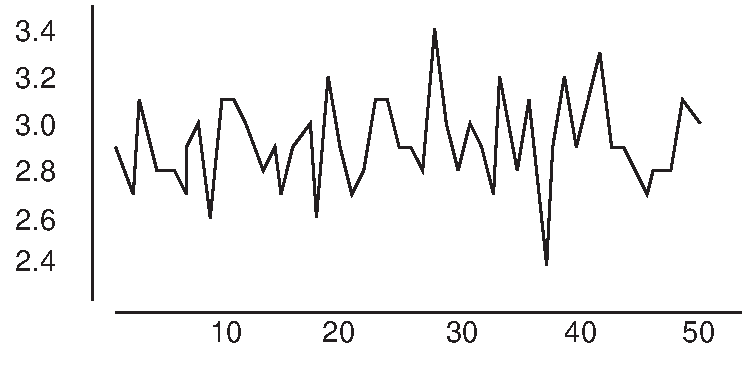
\includegraphics[scale=0.8]{figurer/fig1_5.pdf}
\caption{Tidsplott}
	\label{fig:Tidsplott}
\end{figure}

Plottet gir inntrykk av at kvaliteten varierer tilfeldig omkring nivået
2.9 gjennom hele uken.  Dette fordi ingen dag (eller del av dag) ser ut til
å peke seg ut som annerledes enn de andre, og det heller ikke ser ut
til at en eller flere observerte gode (evt.dårlige) prøver gir
kunnskap om hvor neste prøve plasserer seg i forhold til 
gjennomsnittsnivået.  Merk at dette spørsmål ikke ble avklart
i Eksempel 6.

Når prosessen varierer tilfeldig (uavhengighet) under like forhold hele
tiden (tidshomogenitet), sier vi at prosessen er i ``statistisk kontroll''.
Forstå\-else av slike prosesser er nødvendig for å analysere mer
kompliserte pro\-sesser fra virkeligheten.  For å overvåke 
produksjonssystemer og administrative systemer, trengs metoder til å
avgjøre om en prosess er i kontroll eller ikke.  For økonomiske
tidsrekker trengs kjennskap til ulike former for avhengighet, når en
skal lage prognoser og vurdere påliteligheten av disse.  Dette er spørsmål
som tas opp i Kapittel 13 og 15 påggrunnlag av kunnskaper fra Kapittel 1-8.
\end{eksempel}

Det er ikke alltid lett å gjennomskue tilfeldighetenes rolle 
ved sta\-tistiske undersøkelser og i studiet av prosesser som omgir oss.
For å oppnå en grunnforståelse kan simuleringseksperimenter
være et nyttig hjelpemiddel.  Myntkast er den enkleste form for slik
eksperimentering, og er godt egnet til å klarlegge ulike sider
ved tilfeldighetsbegrepet, som kan komme oss til nytte også i mer praktiske
situasjoner (se Oppgave~14).

Teoretisk statistikk er i hovedsak å lage og utnytte modeller som
knytter observasjonene til det fenomen vi er interessert i.
Siden vi typisk ønsker å
vurdere risikoen for feilkonklusjoner, vil dette som regel være en
stokastisk modell. Studium av slike modeller kan også gi
forståelse av hva slags observasjoner som bør innhentes, samt
en vurdering av ulike analysemetoder. Hva slags modeller som er
aktuelle i en gitt situasjon, vil kunne variere betydelig med
det problemområde det er tale om, men det er likevel mulig å
gi visse basiskunnskaper av almen karakter. Selv om de
situasjonene som er tatt som eksempel ovenfor kan
synes relativt enkle, kan en neppe vente å finne endelig svar på alle
spørsmål innenfor teorirammen i en elementær lærebok. 
Kunnskaper herfra gjør det imidlertid mulig å orientere seg mot spesiallitteratur.

\section{Oppgaver}
\small
\begin{enumerate}
\item
Ta for deg en mynt, knips den $n$=100 ganger og observer antall
kron. Er det noen grunn til å anta at den ikke er rettferdig?
\item
Ta for deg en tegnestift og kast den ut på bordet gjentatte
ganger og observer om den faller til ro med spissen i været eller
ikke. Beregn hyppigheten av spiss i været etter $n$=10,20,30,\ldots,100
kast. Ser det ut til at hyppigheten stabiliseres etter hvert?
Tør du uttale deg noe om sjansen for at spissen peker i været ved
et enkelt kast? Overlat stiften til en annen og be ham/henne
gjenta forsøksserien. Sammenlign de erfaringer som gjøres.
\item
Per og Pål kaster to vanlige mynter og vil observere antall kron.
De er uenige om sjansen for å få resultatene $r_{1}$=ingen kron,
$r_{2}$=en kron og $r_{3}$=to kron. Per foreslår at sjansene er henholdsvis
$\frac{1}{3},\frac{1}{3},\frac{1}{3}$, mens Pål foreslår
$\frac{1}{4},\frac{1}{2},\frac{1}{4}$. Hvem støtter du?
Hvis du er usikker forsøk med litt myntkasting.
\item
Vurder sjansen for regn i morgen. Hvordan skulle et utsagn om at
sjansen for regn er 60\% eventuelt kunne tolkes?
\item
I veiledningen til en meningsmåling om tilslutningen til politiske
partier står det at feilmarginer man må regne med er 2-3\% hver vei,
størst for de største partiene. Hva legger du i denne veiledning?
\item
Etter jordskjelvet i San Francisco-området høsten 1989, ble det uttalt
at sannsynligheten for et større jordskjelv før år 2000 var 50\%.
Hva legger du i denne opplysningen?
Vil du oppfatte et tilsvarende utsagn om oljeutblåsning i Nordsjøen
annerledes?
\item
Følg med i en dagsavis i en uke, og let etter ord som sannsynlig og
sannsynlighet, samt eventuelle betraktninger knyttet til sannsynligheter.
Er det grunn til å tro at ordene er brukt i en mer presis betydning
enn den dagligdagse?
Les Lottokommentarene i en tabloidavis, for å sjekke om journalisten

har en adekvat forståelse av tilfeldighetens rolle.

\item
Forsøk pilkast mot en sirkulær skive med poengskala, f.eks. fra 0 til 5.
Noter resultatet i hvert av $n$=30 kast. Lag hyppighetsfordeling og
tegn histogram. Beregn gjennomsnitt og standardavvik. Gjenta
eksperimentet med en lengre avstand fra skiven. Hva erfarer du?
\item
Bruk dataene i Eksempel 7 til å vinne egen erfaring om påliteligheten
av stikkprøver. For å velge ut studenter kan du bruke en terning.
La f.eks. utfallet av tre etterfølgende kast bestemme nr. på
henholdsvis boks, linje og søyle i tabellen. Gjør gjentatte forsøk
med ulike stikkprøvestørrelser, f.eks. $n$=5 og $n$=10.
I tillegg til å anslå gjennomsnittsverdien i populasjonen kan du
også prøve å anslå medianverdien i populasjonen, f.eks. ved å bruke
medianen i stikkprøven (den midterste når n er oddetall, og 
gjennomsnittet av de to midterste når n er partall). 
\item
Spør noen av dine venner (8-10 er nok) om deres høyde ($X$) og
vekt ($Y$). Beregn korrelasjonskoeffisienten mellom $X$ og $Y$.
Tegn observasjonene i et spredningsdiagram, og legg inn minste
kvadraters regresjonslinjen for $Y$ mhp. $X$. Kommenter.
\item
Undersøk tilgjengelige lommeregnere om muligheten for lettvint
beregning av gjennomsnitt, standardavvik og eventuelt kovarians
(f.eks. med egne taster). Det kan vises at

\[S_{X}^{2}=\frac{1}{n}\sum_{i=1}^{n} X_{i}^{2}-\bar{X}^{2} \]
\[S_{XY}=\frac{1}{n}\sum_{i=1}^{n} X_{i}Y_{i}-\bar{X}\cdot\bar{Y} \]

Kan dette forenkle utregningene i forhold til de opprinnelige 
formlene?

\item
Ved en bedrift er det observert forurensingsgrad for ulike aktivitetsnivåer
(f.eks. antall ovner i drift) ved 12 tidspunkter. Resultatet ble :
\begin{center} \addtolength{\tabcolsep}{-0.5\tabcolsep}
\begin{tabular}{lcccccccccccc}
Aktivitetsnivå :&3&5&2&4&2&1&3&1&2&5&4&3 \\ 
Forurensingsgrad : &4.7&6.4&3.5&5.4&3.9&2.6&5.9&4.1&5.1&4.6&6.1&3.0
\end{tabular}
\end{center}
Plott forurensingsgrad mot aktivitetsnivå. Beregn beskrivende mål.
Beregn regresjonslinjen, og tegn den inn i plottet. Vurder muligheten for
å predikere forurensingsgrad.

\item
For en produksjonsprosess er det observert kvalitet for en stikkprøve

tatt fra $n$=50 etterfølgende perioder, jfr. Eksempel 10.

Resultatet ble (med en desimal) :

\begin{center}
\begin{tabular}{cccccccccc}

2.9&3.0&3.1&3.0&2.9&3.1&3.4&3.0&3.0&2.9 \\
2.9&3.0&2.9&3.0&3.1&2.7&2.6&2.7&2.7&2.4 \\
2.7&2.6&2.7&2.8&2.7&2.8&2.8&2.8&2.9&2.8 \\
2.8&2.9&2.9&2.9&2.8&2.8&2.8&2.9&2.9&2.8 \\
3.2&3.1&3.1&3.1&3.2&3.3&3.1&2.9&3.2&3.1 \\
\end{tabular}
\end{center}
Lag et tidsplott og vurder om prosessen er i kontroll.  Hvis ikke, tenk over
mulige årsaker.
\item
Folk legger ofte merke til spesielle resultater i gjentatte eksperimenter,
som de tviler på er rene tilfeldigheter, eller handler som om det ikke
var det.  Eksempler på beslektede situasjoner er:

\begin{itemize}
\item[-]   Mange kron på rad i myntkast.
\item[-]   Fravær av sekser i terningkast (LUDO)
\item[-]   Samme siffer (eller fravær av et siffer) i mange Lottoomganger
           på rad.
\item[-]   Mange utskiftninger av lyspærer rett etter hverandre.
\end{itemize}

Bruk myntkastresultatene fra Oppgave~1 til å undersøke 
tilfeldigheters rolle ved å studere

\begin{itemize}
\item [(a)] hvor ofte lange serier med kron forekommer
\item [(b)] hyppigheten av kron etter en kron, to kron osv.
\end{itemize}



Vil du etter seks røde i rulett (i) satse rødt (``i siget''),
(ii) satse sort (``rødt hell er oppbrukt``), (iii) satse likegyldig eller
(iv) la være å satse?

\item
Nedenfor er gitt en typisk utskrift fra statistisk programvare der beskrivende
mål for dataene i Eksempel 7 er beregnet.
\begin{center} \framebox[10cm]{\begin{minipage}{9cm}\rule[-0.5cm]{0cm}{0.5cm}
\tt 

 >> READ 'eks1.7' 'Beloep'\\
 >> DESCRIBE 'Beloep' \\
\begin{tabular}{lrrrrrr}
              &      N &    Mean &  Median & StDev &   Min & Max \\
 Beloep       &    216 &   143.7 &   85.52 & 155.2 &     0 & 846 \\
 \end{tabular}
\end{minipage}} \end{center}
\begin{enumerate}
\item
Bruk tilgjengelig programvare til å reprodusere disse resultatene.
\item
Gir din programvare flere beskrivende mål enn de som er med her?
\item
Bruk din programvare til å beregne beskrivende mål for dataene
i Eksempel 8, herunder korrelasjonen mellom karakterene i de to fagene.
\end{enumerate}
Oppgaven forutsetter at filer med dataene er tilgjengelige. Hvis dette ikke er
tilfelle, løs oppgaven med et utvalg på 10 tilfeldig valgte observasjoner.
som leses inn for hånd.


\item
Programvare gir typisk mulighet for tilfeldige trekninger, her illustrert med
uttrekning av 10 studenter blant populasjonen på 216 i Eksempel 7.
\begin{center} \framebox[10cm]{\begin{minipage}{9cm}\rule[-0.5cm]{0cm}{0.5cm}
\tt 

 >> SET 'Populasjon'; DATA 1:216.\\
 >> SAMPLE 10 from 'Populasjon' put into 'Utvalg'\\
 >> PRINT 'Utvalg' \\
    47 12 118 200 77 33 115 10 127 151 \\
\end{minipage}} \end{center}
\begin{enumerate}
\item
Bruk tilgjengelig programvare til å lage en populasjon med studentnumre fra
1 til 216, og trekk så et utvalg på 10 numre.
\item
Hvis vi bare var interessert i beløpene, kan vi isteden trekke fra en
populasjon med disse. Hvordan kan du få til det?
\end{enumerate}

\end{enumerate}

\noindent
{\bf Merknad:} Kommandoer og utskrifter i denne boken ligner de vi finner i
Minitab (som anbefales), men er redigert noe for at leseren lettere skal finne
sammenhengen med teksten i boken forøvrig.

\normalsize

             
   
